\documentclass[11pt,a4paper]{article}

\usepackage[utf8]{inputenc}
\usepackage[T1]{fontenc}
\usepackage{lmodern}
\usepackage[margin=2.5cm]{geometry}
\usepackage{amsmath,amssymb,bm}
\usepackage{graphicx}
\usepackage{booktabs}
\usepackage{array}
\usepackage{caption}
\usepackage{enumitem}
\usepackage[hidelinks]{hyperref}

% Nombres en español (sin depender de babel-spanish)
\renewcommand{\contentsname}{Índice}
\renewcommand{\abstractname}{Resumen}
\renewcommand{\figurename}{Figura}
\renewcommand{\tablename}{Tabla}

\graphicspath{{../resultados_batadal/figuras_optuna_colab/}{../resultados_batadal/optuna_colab_final/}{../resultados_batadal/optuna_colab/}}

\newcommand{\R}{\mathbb{R}}
\newcommand{\A}{\mathbf{A}}
\newcommand{\Ahat}{\hat{\mathbf{A}}}
\newcommand{\X}{\mathbf{X}}
\newcommand{\Z}{\mathbf{Z}}
\newcommand{\E}{\mathbb{E}}
\newcommand{\UCL}{\mathrm{UCL}}
\DeclareMathOperator{\KL}{KL}
\DeclareMathOperator{\diag}{diag}

\title{Detección de ciberataques en la red C-Town (BATADAL)\\[4pt]
\large Metodología y fundamentos teóricos del modelo VGAE + SPC}
\author{}
\date{}

\begin{document}
\maketitle

\begin{abstract}
Se propone un detector de ciberataques para el sistema de distribución de agua C-Town
que combina un \emph{Variational Graph Autoencoder} (VGAE) con cartas de Control
Estadístico de Procesos (SPC). Los sensores del sistema SCADA se representan como
nodos de un grafo construido a partir de la topología hidráulica y de la lógica de
control de la red. El VGAE se entrena únicamente con operación normal y aprende a
reconstruir ventanas temporales de cada sensor; durante la operación, el error de
reconstrucción se vigila con una carta EWMA sobre un estadístico estandarizado por
sensor y con la carta SPE, y el espacio latente con el $T^2$ de Hotelling. Los
hiperparámetros del modelo y de
la carta se seleccionan con optimización bayesiana (TPE) sobre un conjunto de
validación con ataques, y la evaluación final se realiza sobre el conjunto de prueba
de BATADAL sin reajuste.
\end{abstract}

\tableofcontents
\newpage

%=====================================================================
\section{Planteamiento del problema}
%=====================================================================

Sea $\mathbf{x}_t\in\R^{N}$ el vector de lecturas SCADA en la hora $t$. El objetivo es
construir una regla $\hat y_t\in\{0,1\}$ que indique si en el instante $t$ el sistema
está bajo ataque, usando solo información disponible hasta $t$. El problema se aborda
como \emph{detección de anomalías semisupervisada}: el modelo aprende la distribución
de la operación normal y se declara una alarma cuando las observaciones se apartan
de ella de forma estadísticamente significativa. Los datos etiquetados con ataques se
usan exclusivamente para elegir hiperparámetros y para evaluar.

Esta formulación responde a dos características del problema: (i) los ataques son
escasos y heterogéneos (manipulación de actuadores, de lecturas o ambos, con
ocultamiento en algunos casos), por lo que un clasificador supervisado tendería a
memorizar los ataques vistos; y (ii) los sensores no son independientes, sino que
están acoplados por la física hidráulica y por los lazos de control de los PLC, y
un ataque suele romper precisamente esas relaciones.

%=====================================================================
\section{Datos}
%=====================================================================

\subsection{Conjuntos de BATADAL}

El \emph{BATtle of the Attack Detection ALgorithms} (BATADAL) proporciona series
horarias simuladas con EPANET sobre la red C-Town (\texttt{CTOWN.INP}), con 7
tanques, 11 bombas, 1 válvula y 388 nodos de demanda. Se usan tres conjuntos
(Tabla~\ref{tab:datos}).

\begin{table}[h]
\centering
\caption{Conjuntos de datos y su uso en el protocolo.}
\label{tab:datos}
\begin{tabular}{@{}lrrl@{}}
\toprule
Conjunto & Horas & Horas en ataque & Uso \\
\midrule
\texttt{dataset03} (80\,\% inicial) & 7\,008 & 0 & Entrenamiento del VGAE \\
\texttt{dataset03} (20\,\% final)  & 1\,753 & 0 & Validación y Fase~I del SPC \\
\texttt{dataset04} & 4\,177 & 492 (ataques 1--7) & Selección de hiperparámetros \\
Prueba & 2\,089 & 407 (ataques 8--14) & Evaluación final \\
\bottomrule
\end{tabular}
\end{table}

Las etiquetas de \texttt{dataset04} provistas en el CSV están incompletas (parte de
los ataques se marcó como desconocida), por lo que se reconstruyeron las ventanas
completas de cada ataque a partir de la documentación oficial
(\texttt{Attacks\_TrainingDataset4.png} y \texttt{Attacks\_TestDataset.png}). Así,
cada hora tiene una etiqueta $y_t\in\{0,1\}$ y un identificador de ataque.

\subsection{Variables y preprocesamiento}

Las 43 señales originales son: niveles de tanque ($L\_T1$--$L\_T7$), caudal y estado
de bombas ($F\_PUi$, $S\_PUi$), caudal y estado de la válvula ($F\_V2$, $S\_V2$) y
12 presiones de succión/descarga en uniones ($P\_J\ast$). Se eliminan las 7 señales
con varianza nula en operación normal (bombas PU3, PU5 y PU9, que nunca operan, y
$S\_PU1$, siempre encendida), pues no aportan información y harían indefinida la
estandarización. Quedan $N=36$ sensores.

Cada señal se estandariza con la media y desviación típica del tramo de
entrenamiento ($80\,\%$ inicial de \texttt{dataset03}):
\begin{equation}
\tilde x_{t,i} = \frac{x_{t,i}-\bar x_i}{s_i}.
\end{equation}
Los parámetros se estiman solo con datos de entrenamiento para evitar fuga de
información hacia la Fase~I, \texttt{dataset04} y la prueba.

\subsection{Ventanas deslizantes}

La entrada al modelo en el instante $t$ es la matriz de atributos de nodo
\begin{equation}
\X_t = \big[\tilde{\mathbf{x}}_{t-W+1},\dots,\tilde{\mathbf{x}}_{t}\big]
\in\R^{N\times W},
\end{equation}
es decir, cada nodo (sensor) lleva como vector de atributos las últimas $W$ horas de
su propia señal. La ventana que termina en $t$ es causal: solo usa el pasado, por lo
que la detección puede ejecutarse en línea. Las primeras $W-1$ horas de cada serie no
tienen puntuación y se consideran sin alarma.

%=====================================================================
\section{Grafo de sensores}
%=====================================================================

\subsection{Motivación}

Un autoencoder convencional trata el vector de sensores como un conjunto sin
estructura. En una red de agua, sin embargo, las relaciones entre sensores son
conocidas a priori: el caudal de una bomba y su estado están ligados, la presión de
descarga depende de la bomba que la alimenta y el nivel de un tanque gobierna,
mediante reglas del PLC, el arranque de ciertas bombas. Codificar ese conocimiento en
un grafo $\mathcal{G}=(\mathcal{V},\mathcal{E})$ con $|\mathcal{V}|=N$ permite que el
modelo reconstruya cada sensor a partir de sus vecinos físicamente relacionados, y que
la manipulación de un sensor (que rompe su coherencia con los vecinos) produzca un
error de reconstrucción localizado.

\subsection{Construcción}

A partir de \texttt{CTOWN.INP} se construye un grafo hidráulico ponderado cuyas
aristas son las tuberías (peso = longitud) y las bombas y válvulas (peso unitario).
Cada sensor se ubica en un nodo de esa red: los niveles en su tanque, las presiones
en su unión y los sensores de bombas/válvulas en su nodo de succión. Con el algoritmo
de Dijkstra se obtiene la distancia hidráulica $D_{ij}$ entre todos los pares de
sensores. La matriz de adyacencia binaria y simétrica $\A\in\{0,1\}^{N\times N}$
(sin bucles) se forma con la unión de cuatro tipos de arista:

\begin{enumerate}[label=(\roman*)]
\item \textbf{Mismo dispositivo:} caudal $\leftrightarrow$ estado del mismo equipo
  (p.\,ej.\ $F\_PU2$--$S\_PU2$).
\item \textbf{Estación de bombeo:} presiones y sensores de bombas/válvulas cuya
  distancia hidráulica es $D_{ij}\le 5$\,m, es decir, que pertenecen a la misma
  estación.
\item \textbf{Lazos de control:} nivel de tanque $\leftrightarrow$ actuadores que lo
  controlan según la sección \texttt{[CONTROLS]} del archivo de red
  (T1$\to$PU1, PU2; T2$\to$V2; T3$\to$PU4, PU5; T4$\to$PU6, PU7; T5$\to$PU8;
  T7$\to$PU10, PU11).
\item \textbf{$k$ vecinos hidráulicos:} cada sensor se une a los $k$ sensores de otro
  dispositivo más cercanos en distancia $D_{ij}$.
\end{enumerate}

Los tres primeros tipos son fijos; $k$ es un hiperparámetro. Con $k=1$ (configuración
seleccionada) el grafo tiene 65 aristas: 8 de dispositivo, 24 de estación, 17 de
control y 16 hidráulicas (Figura~\ref{fig:grafo}). Como varios sensores comparten
ubicación (p.\,ej.\ las bombas de una misma estación), existen empates de distancia
en el paso (iv); el desempate se fija ordenando de forma estable y la adyacencia
usada en el entrenamiento se guarda junto con el modelo para que la evaluación use
exactamente el mismo grafo.

\begin{figure}[t]
\centering
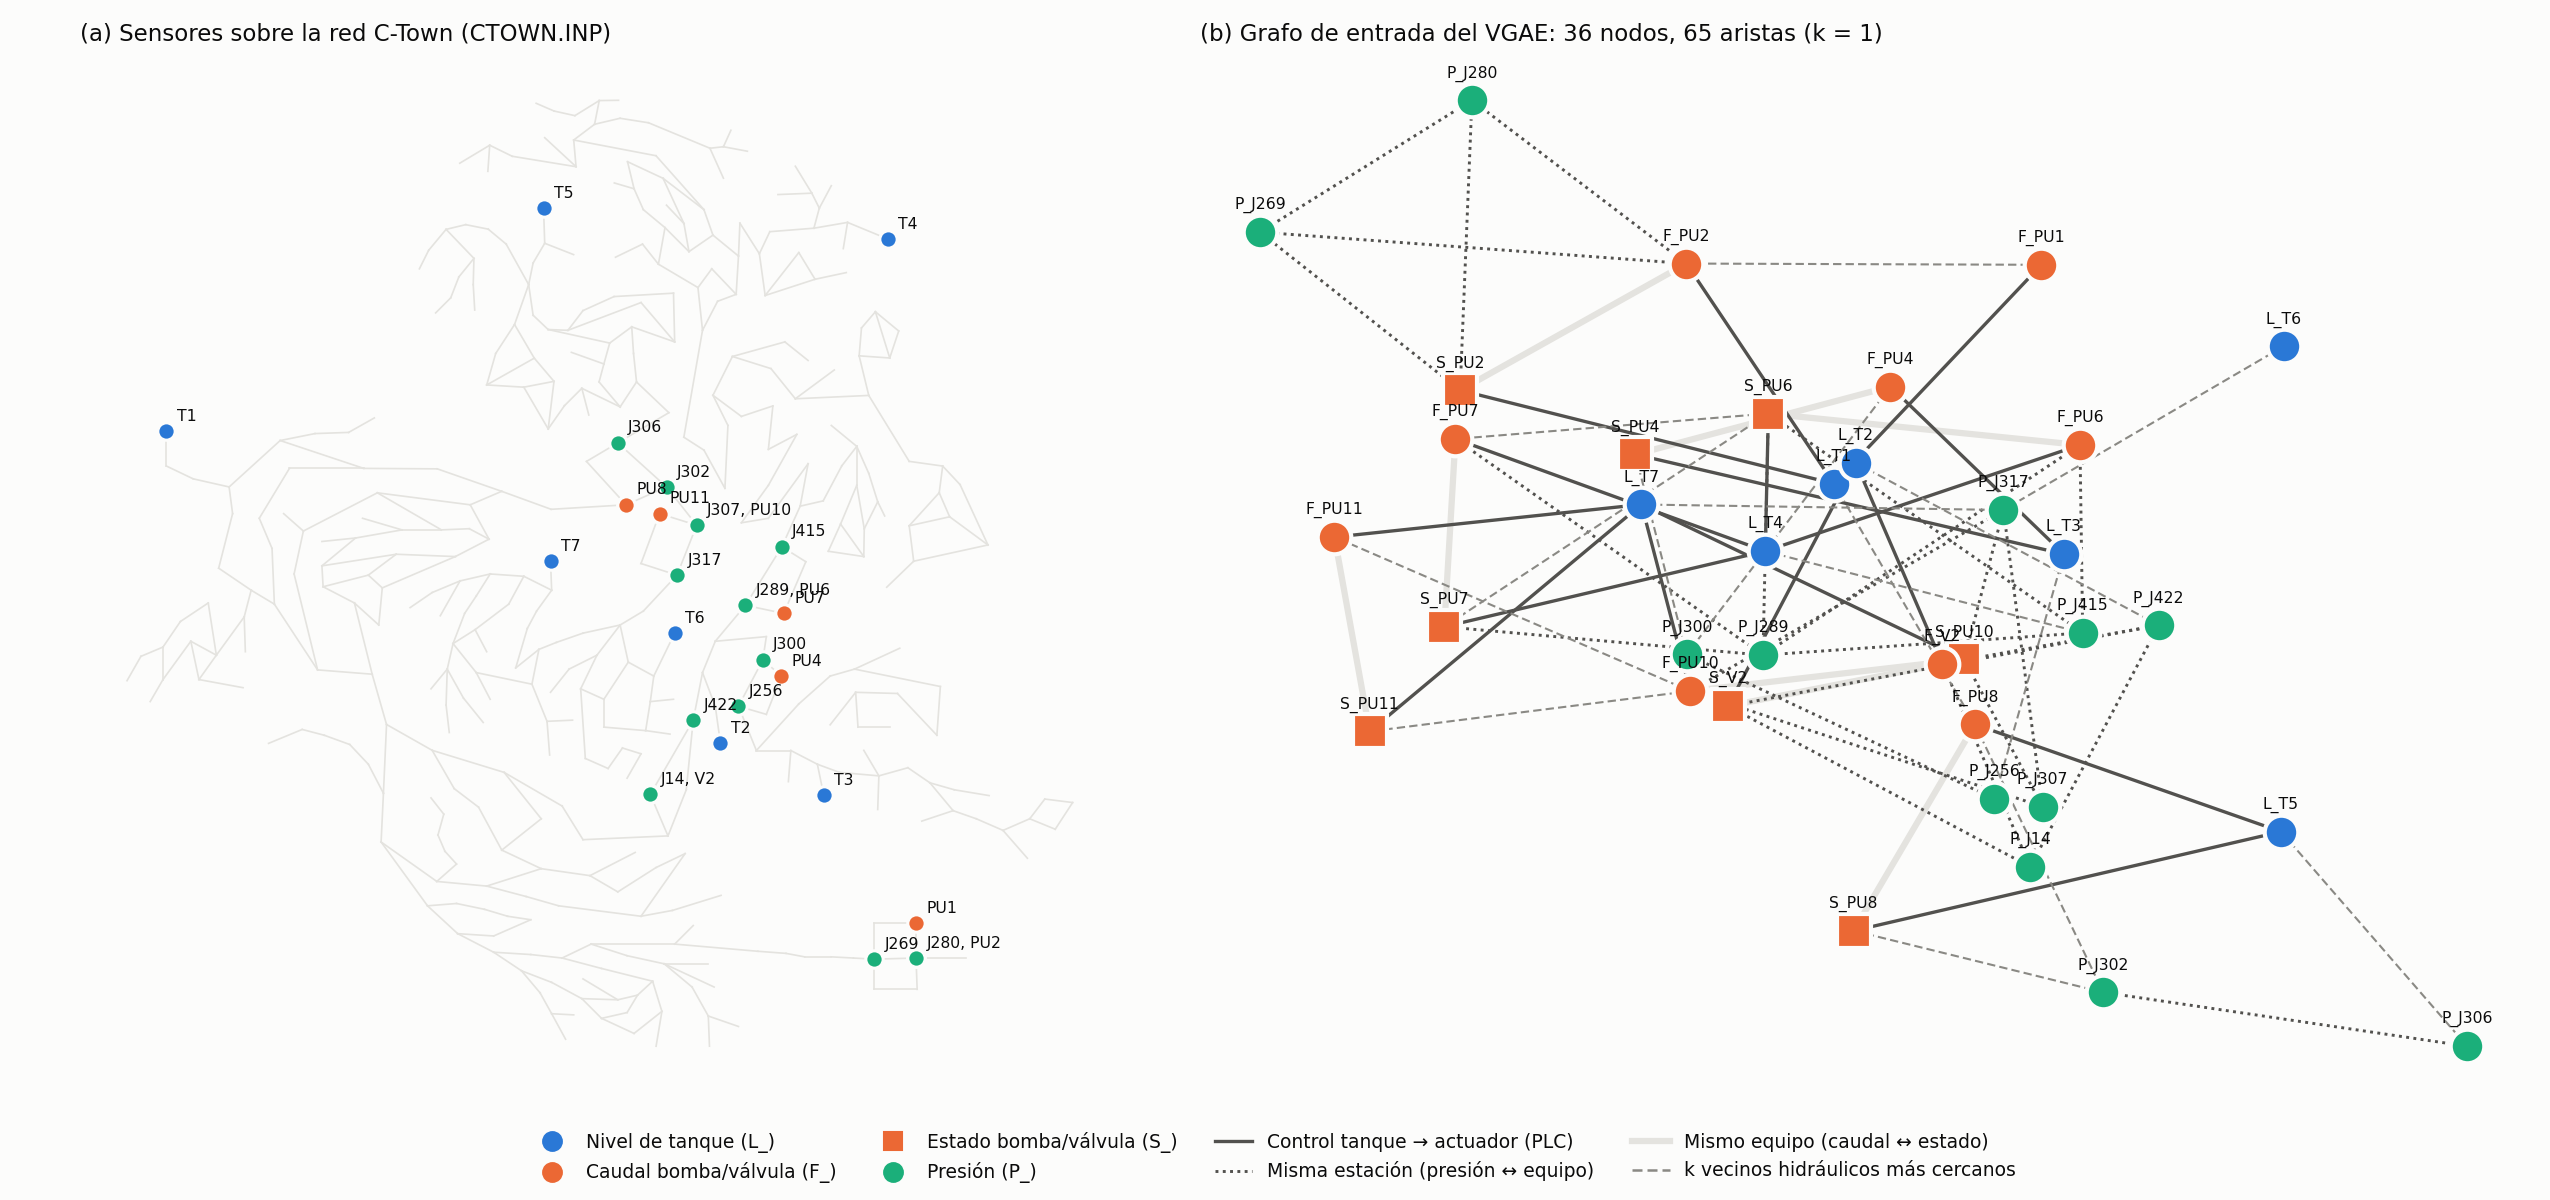
\includegraphics[width=\textwidth]{grafo_sensores.png}
\caption{(a) Ubicación de los sensores en la red C-Town. (b) Grafo de entrada del
VGAE con los cuatro tipos de arista.}
\label{fig:grafo}
\end{figure}

%=====================================================================
\section{Fundamentos teóricos del modelo}
%=====================================================================

\subsection{Redes convolucionales sobre grafos}

Una red convolucional de grafos (GCN; Kipf y Welling, 2017) generaliza la convolución
a datos definidos sobre nodos. Partiendo de la convolución espectral con el
laplaciano normalizado y truncando su aproximación de Chebyshev al primer orden, se
obtiene la regla de propagación
\begin{equation}
\mathbf{H}^{(l+1)} = \sigma\!\left(\Ahat\,\mathbf{H}^{(l)}\mathbf{W}^{(l)}\right),
\qquad
\Ahat = \tilde{\mathbf{D}}^{-1/2}(\A+\mathbf{I})\tilde{\mathbf{D}}^{-1/2},
\label{eq:gcn}
\end{equation}
donde $\tilde{\mathbf{D}}=\diag\big(\sum_j(\A+\mathbf{I})_{ij}\big)$. Cada capa
transforma linealmente los atributos de cada nodo y luego los promedia con los de sus
vecinos (incluido él mismo, por los bucles añadidos) con pesos normalizados por el
grado. La normalización simétrica mantiene los autovalores de $\Ahat$ en $(-1,1]$, lo
que estabiliza la propagación al apilar capas. Tras $l$ capas, la representación de
un nodo depende de su vecindario a $l$ saltos.

En la implementación, una capa GCN calcula
$\Ahat(\mathbf{H}\mathbf{W}+\mathbf{b})$ y se aplica de forma independiente a cada
ventana del lote, compartiendo $\Ahat$, que es fijo.

\subsection{Autoencoder variacional}

Un autoencoder variacional (VAE; Kingma y Welling, 2014) es un modelo generativo con
variables latentes $\mathbf{z}$, prior $p(\mathbf{z})=\mathcal{N}(\mathbf{0},\mathbf{I})$
y verosimilitud $p_\theta(\mathbf{x}\mid\mathbf{z})$. Como la posterior exacta es
intratable, se introduce una distribución aproximada $q_\phi(\mathbf{z}\mid\mathbf{x})$
(el \emph{encoder}) y se maximiza la cota inferior de la evidencia (ELBO):
\begin{equation}
\log p_\theta(\mathbf{x}) \;\ge\;
\E_{q_\phi(\mathbf{z}\mid\mathbf{x})}\!\left[\log p_\theta(\mathbf{x}\mid\mathbf{z})\right]
-\KL\!\left(q_\phi(\mathbf{z}\mid\mathbf{x})\,\big\|\,p(\mathbf{z})\right).
\label{eq:elbo}
\end{equation}
El primer término favorece reconstrucciones fieles; el segundo regulariza el espacio
latente acercándolo al prior, lo que produce representaciones suaves y evita que el
modelo memorice cada muestra. Con $q_\phi=\mathcal{N}(\bm\mu,\diag\bm\sigma^2)$ la
divergencia tiene forma cerrada,
\begin{equation}
\KL = -\tfrac12\sum_{d=1}^{D}\left(1+\log\sigma_d^2-\mu_d^2-\sigma_d^2\right),
\end{equation}
y el gradiente respecto a $\phi$ se obtiene con el \emph{truco de
reparametrización}: $\mathbf{z}=\bm\mu+\bm\sigma\odot\bm\varepsilon$,
$\bm\varepsilon\sim\mathcal{N}(\mathbf{0},\mathbf{I})$.

Si la verosimilitud es gaussiana con varianza fija, maximizar el primer término de
\eqref{eq:elbo} equivale a minimizar el error cuadrático medio, y la ponderación del
término KL por un factor $\beta$ ($\beta$-VAE) controla el compromiso entre fidelidad
de reconstrucción y regularidad del espacio latente.

\subsection{Variational Graph Autoencoder}

El VGAE (Kipf y Welling, 2016) combina ambas ideas: el encoder es una GCN que produce
una distribución latente por nodo,
\begin{equation}
q(\Z\mid\X,\A)=\prod_{i=1}^{N}\mathcal{N}\!\left(\mathbf{z}_i\mid\bm\mu_i,\diag\bm\sigma_i^2\right),
\qquad
\bm\mu=\mathrm{GCN}_\mu(\X,\A),\;\;\log\bm\sigma^2=\mathrm{GCN}_\sigma(\X,\A),
\end{equation}
donde ambas cabezas comparten la primera capa. El decoder original reconstruye la
estructura mediante un producto interno,
\begin{equation}
p(A_{ij}=1\mid\mathbf{z}_i,\mathbf{z}_j)=\sigma\!\left(\mathbf{z}_i^\top\mathbf{z}_j\right),
\end{equation}
de modo que nodos conectados deben tener representaciones latentes alineadas.

\subsection{Adaptación al monitoreo de sensores}

En este problema el grafo es fijo y lo que cambia en el tiempo son los atributos de
los nodos. Reconstruir solo $\A$ no daría información sobre el estado del proceso, por
lo que se introducen tres modificaciones al VGAE original.

\paragraph{Decoder de atributos.} Se añade un segundo decoder que reconstruye la
ventana temporal de cada sensor:
\begin{equation}
\hat{\X} = \mathrm{ReLU}\!\left(\Ahat\,[\Z\,\|\,\mathbf{E}]\,\mathbf{W}_d\right)\mathbf{W}_o,
\qquad \hat{\X}\in\R^{N\times W}.
\end{equation}
Al ser también una GCN, el valor reconstruido de un sensor se apoya en el estado
latente de sus vecinos. Si un atacante altera la lectura de un sensor sin alterar
coherentemente la de sus vecinos (o viceversa), la reconstrucción falla
precisamente en ese nodo.

\paragraph{Embeddings de nodo.} La GCN es invariante a permutaciones: dos nodos con
atributos y vecindarios similares reciben la misma representación. Sin embargo, una
presión y un nivel de tanque tienen dinámicas muy distintas. Para que el modelo
distinga la identidad de cada sensor se aprende un vector $\mathbf{e}_i\in\R^{d_e}$
por nodo, que se concatena a la entrada del encoder y a la del decoder de atributos
($\mathbf{E}=[\mathbf{e}_1,\dots,\mathbf{e}_N]^\top$).

\paragraph{Decoder de estructura como regularizador.} Se conserva el decoder de
producto interno, pero con un peso $\alpha$ pequeño: obliga a que el espacio latente
refleje la topología, sin dominar la pérdida.

\paragraph{Arquitectura.} El modelo resultante (Figura~\ref{fig:arq}) es:
\begin{align*}
\mathbf{H} &= \mathrm{ReLU}\big(\Ahat\,[\X\,\|\,\mathbf{E}]\,\mathbf{W}_1\big)
&& (W+d_e)\to h,\\
\bm\mu &= \Ahat\,\mathbf{H}\mathbf{W}_\mu,\quad
\log\bm\sigma^2 = \mathrm{clip}\big(\Ahat\,\mathbf{H}\mathbf{W}_\sigma,\,-10,\,10\big)
&& h\to d_z,\\
\Z &= \bm\mu+\bm\sigma\odot\bm\varepsilon \;\text{(entrenamiento)},\qquad \Z=\bm\mu \;\text{(inferencia)},\\
\hat{\X} &= \mathrm{ReLU}\big(\Ahat\,[\Z\,\|\,\mathbf{E}]\,\mathbf{W}_d\big)\mathbf{W}_o
&& (d_z+d_e)\to h\to W,\\
\hat{A}_{ij} &= \sigma(\mathbf{z}_i^\top\mathbf{z}_j).
\end{align*}
En inferencia se usa la media $\bm\mu$ (sin muestreo), lo que hace el puntaje
determinista.

\begin{figure}[t]
\centering
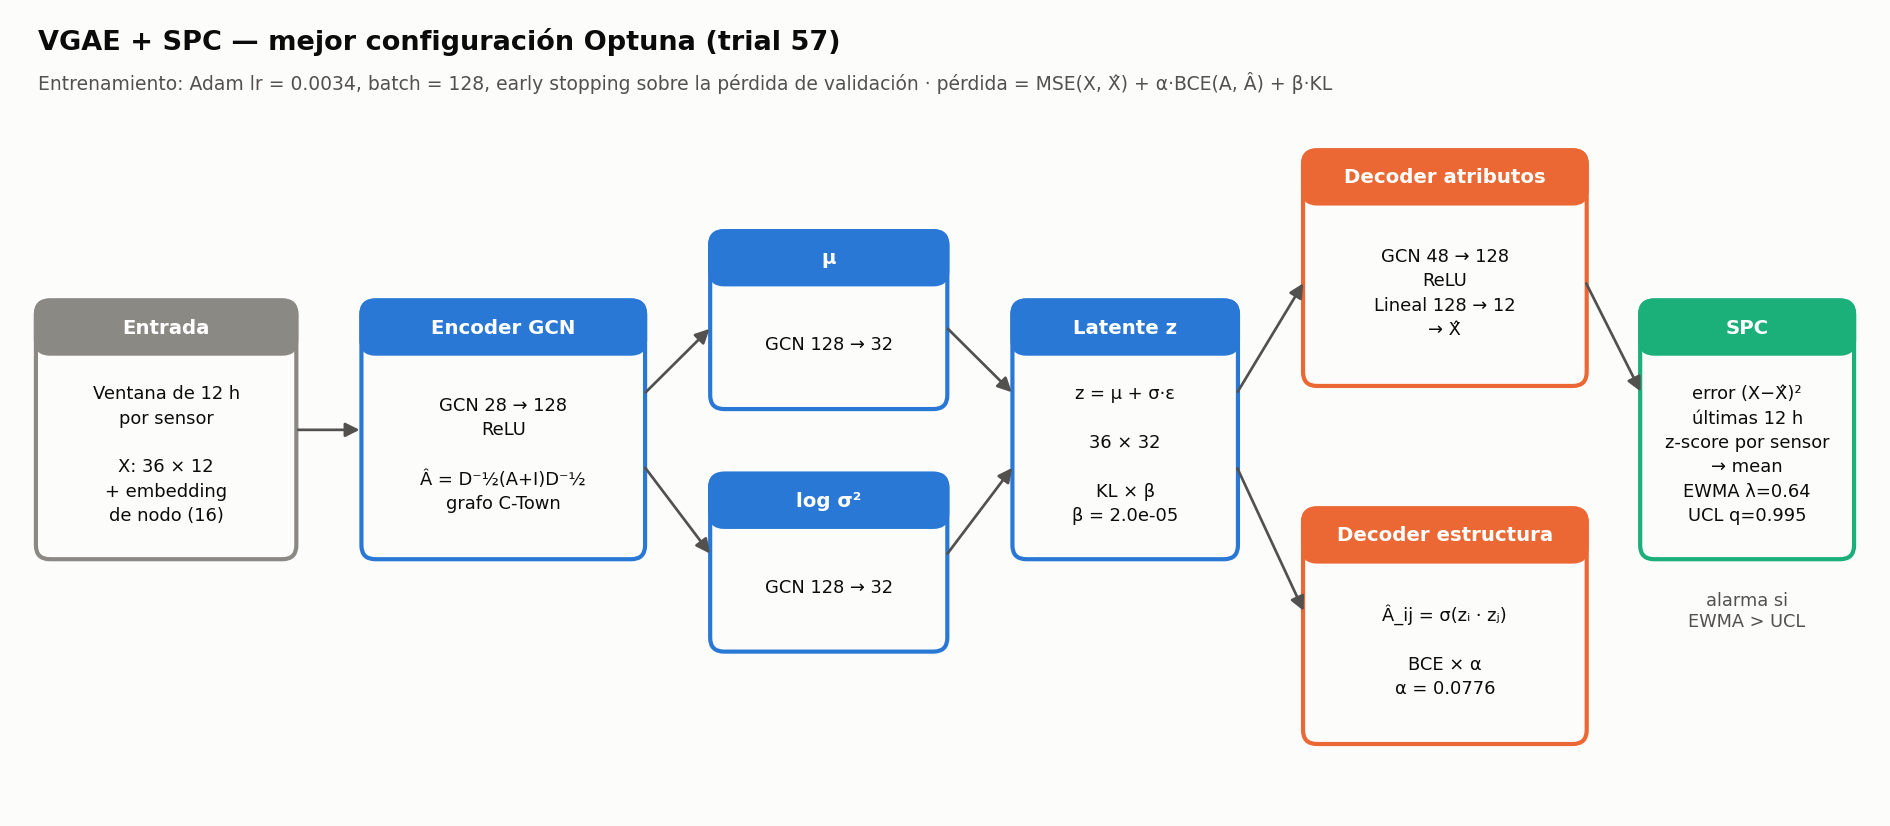
\includegraphics[width=\textwidth]{arquitectura_vgae.png}
\caption{Arquitectura VGAE + SPC con la configuración seleccionada.}
\label{fig:arq}
\end{figure}

\subsection{Variante con convolución temporal}
\label{sec:tcn}

En la arquitectura base, la ventana de $W$ horas de cada sensor entra como un vector
plano de atributos: la primera capa la mezcla con una transformación lineal que no
incorpora el orden temporal ni la invariancia a desplazamientos, el modelo no tiene
memoria entre ventanas y desconoce la hora del día. Para modelar la dimensión
temporal de forma explícita se propone una variante que intercala bloques
convolucionales sobre el eje del tiempo con la convolución de grafo, en la línea de
las redes espacio-temporales STGCN (Yu et al., 2018) y de las redes convolucionales
temporales (TCN; Bai et al., 2018).

\paragraph{Codificación de la hora del día.} La demanda de agua sigue un ciclo diario
que una ventana de 12~h no cubre completo. Cada instante se acompaña de
$\big(\sin(2\pi h/24),\,\cos(2\pi h/24)\big)$, con $h$ la hora, de modo que el modelo
conoce la fase del ciclo sin depender solo de los valores observados. La codificación
circular evita la discontinuidad entre las 23~h y las 0~h.

\paragraph{Encoder temporal.} Para cada sensor $i$, la serie de la ventana y la hora
del día forman una señal de 3 canales y longitud $W$, que pasa por una pila de
convoluciones 1D dilatadas con conexión residual:
\begin{equation}
\mathbf{u}^{(b)} = \mathrm{ReLU}\!\left(\mathrm{Conv1D}_{k=3,\,d_b}\big(\mathbf{u}^{(b-1)}\big)
+ \mathbf{P}_b\,\mathbf{u}^{(b-1)}\right),\qquad d_b\in\{1,2,4\},
\end{equation}
donde $\mathbf{P}_b$ es una proyección $1\times1$ cuando cambia el número de canales.
Con núcleo 3 y dilataciones 1, 2 y 4, el campo receptivo es
$1+2(1+2+4)=15\ge W$, por lo que cada posición ve la ventana completa. A diferencia de
la capa lineal, los filtros se comparten a lo largo del tiempo (invariancia a
desplazamientos) y respetan el orden de las horas. La salida, $C=16$ canales por
instante, se aplana a un vector de $C\cdot W$ atributos por nodo, que sustituye a la
ventana cruda como entrada de la GCN; el resto del encoder no cambia.

\paragraph{Decoder temporal.} El decoder de atributos aplica el bloque espejo: la
salida de la GCN se proyecta a $C\cdot W$, se reorganiza como $C$ canales de longitud
$W$, se concatena con la hora del día y pasa por convoluciones dilatadas
($d=4,2,1$) y una convolución $1\times1$ que devuelve un canal: la ventana
reconstruida $\hat{\mathbf{x}}_i\in\R^{W}$.

\paragraph{Qué no cambia.} El grafo, la normalización $\Ahat$, el espacio latente, la
función de pérdida, el estadístico por sensor y las cartas de control son idénticos,
lo que permite atribuir cualquier diferencia de desempeño al tratamiento del tiempo.
La variante tiene unos 71\,000 parámetros frente a 20\,000 del modelo base.

\subsection{Función de pérdida}

Para un lote de ventanas, la pérdida es
\begin{equation}
\mathcal{L} =
\underbrace{\frac{1}{NW}\big\|\X-\hat{\X}\big\|_F^2}_{\text{atributos (MSE)}}
+\alpha\,\underbrace{\mathrm{BCE}_{w}\big(\A,\sigma(\Z\Z^\top)\big)}_{\text{estructura}}
+\beta\,\underbrace{\frac1N\sum_{i=1}^{N}\KL\big(q(\mathbf{z}_i)\,\|\,\mathcal{N}(\mathbf{0},\mathbf{I})\big)}_{\text{regularización}},
\label{eq:loss}
\end{equation}
promediada sobre el lote. La entropía cruzada binaria se pondera con
$w=(N^2-\sum_{ij}A_{ij})/\sum_{ij}A_{ij}$ en las entradas positivas para compensar la
dispersión del grafo (hay muchas más no-aristas que aristas). Esta pérdida es el
negativo de una ELBO con verosimilitud gaussiana para los atributos, Bernoulli para
la estructura y pesos $\alpha,\beta$ en los dos últimos términos.

\subsection{Por qué el error de reconstrucción detecta ataques}

El modelo se entrena solo con operación normal, de modo que aprende la variedad de
baja dimensión en la que viven las ventanas normales y las correlaciones entre
sensores vecinos. Una ventana anómala cae fuera de esa variedad: el encoder la
proyecta sobre el código latente normal más cercano y el decoder devuelve una
versión ``normal'' de la ventana. La diferencia
\begin{equation}
\mathbf{R}_t = (\X_t-\hat{\X}_t)^{\odot 2}\in\R^{N\times W}
\end{equation}
mide la desviación respecto al comportamiento aprendido, con resolución por sensor y
por hora. Dado que el grafo condiciona la reconstrucción, el error no solo detecta
valores atípicos aislados, sino también inconsistencias entre sensores que por
separado parecen normales (por ejemplo, un nivel de tanque falsificado que no
concuerda con el caudal de las bombas que lo alimentan).

%=====================================================================
\section{Control estadístico de procesos sobre las salidas del VGAE}
%=====================================================================

El VGAE proporciona residuos y representaciones latentes; el SPC proporciona la regla
de decisión con una tasa de falsas alarmas controlada. Todas las cartas se calibran en
\emph{Fase~I} (20\,\% final de \texttt{dataset03}: operación normal que el modelo no
usó para ajustar sus pesos) y se aplican en \emph{Fase~II} (\texttt{dataset04} y
prueba).

\subsection{Criterios para elegir las cartas}

\paragraph{Qué se vigila: residuo y espacio latente.} En el monitoreo multivariante
basado en PCA (Jackson y Mudholkar, 1979; Kourti y MacGregor, 1995) se usan dos
estadísticos complementarios: el error de predicción $Q$ (SPE), que detecta
observaciones que \emph{rompen la estructura de correlación} aprendida, y el $T^2$ de
Hotelling sobre las componentes principales, que detecta observaciones
\emph{coherentes con esa estructura pero en una zona inusual} del subespacio del
modelo. El VGAE cumple el papel del PCA, de forma no lineal y respetando el grafo, por
lo que se mantiene la misma lógica:
\begin{itemize}
\item \textbf{Residuo} (EWMA y SPE). Un ataque que falsifica lecturas (p.\,ej.\ un
  nivel de tanque que no concuerda con los caudales de sus bombas) rompe la coherencia
  física entre sensores vecinos y eleva el error de reconstrucción.
\item \textbf{Espacio latente} ($T^2$). Un ataque que manipula actuadores o consignas
  del PLC puede producir una operación físicamente coherente (el modelo la reconstruye
  bien) pero en un régimen anormal; este caso se refleja en el estado latente.
\end{itemize}

\paragraph{Qué tipo de desviación: memoria en la carta del residuo.} Los ataques de
BATADAL, en particular los que ocultan la manipulación, producen desviaciones
moderadas que se sostienen durante horas o días. Las cartas sin memoria son poco
sensibles a este tipo de desplazamiento (Montgomery, 2019, cap.~9), por lo que para el
estadístico del residuo se usa una EWMA, que acumula evidencia en el tiempo.

\paragraph{Cartas descartadas.}
\begin{itemize}
\item \textbf{Shewhart}: es el caso particular $\lambda=1$ de la EWMA. Ese valor se
  incluye en la búsqueda de $\lambda$, de modo que si los datos favorecieran una carta
  sin memoria la búsqueda lo seleccionaría; calcularla por separado es redundante. Como
  referencia se reporta la mejor configuración de la rejilla con $\lambda=1$.
\item \textbf{CUSUM}: para detectar desplazamientos pequeños y sostenidos de la media
  su desempeño es prácticamente equivalente al de la EWMA (Lucas y Saccucci, 1990),
  por lo que no aporta información adicional y añadiría un parámetro más ($k$) que
  ajustar con los mismos datos.
\end{itemize}

\subsection{Estadístico por sensor}
\label{sec:zscore}

Para cada sensor $i$ se promedia el error de reconstrucción de las últimas $L$ horas
de la ventana, se toma logaritmo y se estandariza con la media $m_i$ y desviación
$s_i$ observadas en Fase~I:
\begin{equation}
r_{t,i}=\frac1L\sum_{\ell=W-L+1}^{W}R_{t,i\ell},\qquad
z_{t,i}=\frac{\log(r_{t,i}+10^{-6})-m_i}{s_i}.
\label{eq:zscore}
\end{equation}
\begin{itemize}
\item El \textbf{horizonte} $L\le W$ enfoca el estadístico en las horas más
  recientes, que son las relevantes para una detección temprana.
\item El \textbf{logaritmo} reduce la fuerte asimetría a la derecha del error
  cuadrático y acerca su distribución a la normal.
\item La \textbf{estandarización por sensor} hace comparables sensores con niveles de
  error muy distintos; sin ella, unos pocos sensores difíciles de reconstruir
  dominarían el estadístico y un ataque localizado (p.\,ej.\ solo sobre $L\_T2$ y
  $V2$) se diluiría entre los 36 nodos.
\end{itemize}

Los $z_{t,i}$ se agregan en un escalar $s_t$ mediante la media (\texttt{mean}), el
máximo (\texttt{max}) o la media de los tres mayores (\texttt{top3}). La media es
sensible a desviaciones moderadas y extendidas; el máximo, a desviaciones fuertes en
un único sensor; \texttt{top3} es un compromiso.

\subsection{Límites de control empíricos}

Los límites teóricos de las cartas clásicas suponen observaciones independientes. Las
series monitoreadas están fuertemente autocorrelacionadas, porque ventanas consecutivas
comparten $W-1$ horas, y aplicar esos límites produciría un exceso de falsas alarmas.
Por ello, para la EWMA y el $T^2$ el límite superior se define como el cuantil
empírico $q$ del estadístico de la carta calculado sobre Fase~I:
\begin{equation}
\UCL = Q_q\big(\{C_t\}_{t\in\text{Fase I}}\big),\qquad q\in\{0.99,\,0.995,\,0.999\},
\end{equation}
lo que fija la tasa nominal de falsas alarmas en $1-q$. Se emite alarma en $t$ si
$C_t>\UCL$.

\subsection{Carta EWMA sobre el residuo}

\begin{equation}
C_t=\lambda s_t+(1-\lambda)C_{t-1},\qquad C_0=\bar s_{\text{Fase I}},\quad \lambda\in(0,1].
\end{equation}
La EWMA es un promedio ponderado de todas las observaciones pasadas con pesos que
decaen geométricamente, $C_t=\lambda\sum_{j\ge0}(1-\lambda)^j s_{t-j}$, con memoria
efectiva de $\approx(2-\lambda)/\lambda$ observaciones: con $\lambda$ pequeño se
acumula evidencia de desplazamientos pequeños y sostenidos, y con $\lambda=1$ se
obtiene la carta de Shewhart. Al promediar, es además robusta a la falta de
normalidad del estadístico (Borror et al., 1999). La carta es \emph{unilateral}: solo
un aumento del error de reconstrucción indica ataque. Es la carta principal del
estudio.

\subsection{Carta $T^2$ de Hotelling sobre el espacio latente}

Cada ventana se resume con el embedding del grafo
$\bar{\bm\mu}_t=\frac1N\sum_i\bm\mu_{t,i}\in\R^{d_z}$ (promedio de las medias
latentes de los nodos) y se mide su distancia de Mahalanobis a la operación normal:
\begin{equation}
T^2_t=(\bar{\bm\mu}_t-\mathbf{m})^\top\mathbf{S}^{+}(\bar{\bm\mu}_t-\mathbf{m}),
\end{equation}
donde $\mathbf{m}$ y $\mathbf{S}$ son la media y la covarianza muestral de
$\bar{\bm\mu}_t$ en Fase~I y $\mathbf{S}^{+}$ su pseudoinversa. El $T^2$ es la
versión multivariante de la carta de Shewhart; usar la distancia de Mahalanobis, y no
la euclídea, tiene en cuenta la correlación entre las dimensiones latentes. Vigila
desplazamientos del estado latente (el régimen en que el modelo ``cree'' que está el
sistema), información que el error de reconstrucción no captura.

\subsection{Carta SPE (estadístico $Q$)}

Es la carta clásica para el residuo en el MSPC: el error cuadrático de predicción
sumado sobre sensores,
\begin{equation}
Q_t=\sum_{i=1}^{N} r_{t,i},
\end{equation}
con el límite de Box (1954), usado en PCA multivariante por Nomikos y MacGregor (1995),
que aproxima la distribución de $Q$ por una $g\,\chi^2_h$ con la media $m$ y la
varianza $v$ de Fase~I:
\begin{equation}
g=\frac{v}{2m},\qquad h=\frac{2m^2}{v},\qquad \UCL=g\,\chi^2_{h}(q).
\end{equation}
Se incluye como referencia frente a la EWMA. Hay que tener en cuenta dos
limitaciones: la aproximación $\chi^2$ supone residuos gaussianos de un modelo
lineal, lo que el VGAE no garantiza, y al sumar el error sin estandarizar, los
sensores con mayor error de reconstrucción dominan el estadístico. El estadístico
estandarizado por sensor de la Sección~\ref{sec:zscore} responde precisamente a esta
segunda limitación.

\subsection{Regla combinada}

Siguiendo la práctica del MSPC de vigilar simultáneamente el residuo y el subespacio
del modelo, se evalúa la regla ``EWMA \textsc{o} $T^2$'', que alarma si cualquiera de
las dos cartas supera su límite.

%=====================================================================
\section{Métrica de evaluación}
%=====================================================================

Se usa la métrica oficial de BATADAL, que combina la rapidez de detección y la
calidad de la clasificación:
\begin{equation}
S=\tfrac12\,S_{\mathrm{TTD}}+\tfrac12\,S_{\mathrm{CM}}.
\end{equation}
\begin{itemize}
\item \textbf{Tiempo hasta la detección.} Para cada ataque $a$ de duración
  $\Delta t_a$ horas, $\mathrm{TTD}_a$ es el número de horas entre su inicio y la
  primera alarma dentro de su ventana ($\mathrm{TTD}_a=\Delta t_a$ si no se
  detecta). Entonces
  \begin{equation}
  S_{\mathrm{TTD}}=1-\frac1{n_A}\sum_{a=1}^{n_A}\frac{\mathrm{TTD}_a}{\Delta t_a}.
  \end{equation}
\item \textbf{Matriz de confusión.} A nivel horario,
  \begin{equation}
  S_{\mathrm{CM}}=\frac{\mathrm{TPR}+\mathrm{TNR}}{2},\qquad
  \mathrm{TPR}=\frac{TP}{TP+FN},\quad \mathrm{TNR}=\frac{TN}{TN+FP}.
  \end{equation}
\end{itemize}
Se reportan además precisión, $F_1$ y número de ataques detectados.

%=====================================================================
\section{Protocolo experimental}
%=====================================================================

\subsection{Entrenamiento}

El VGAE se entrena con Adam minimizando \eqref{eq:loss} sobre las ventanas del
80\,\% inicial de \texttt{dataset03}, en mini-lotes barajados en cada época. Se
aplica \emph{early stopping} sobre la pérdida en el 20\,\% final (hasta 300 épocas,
paciencia de 25) y se restauran los pesos de la mejor época. Ese mismo tramo,
que el optimizador nunca ve, sirve como Fase~I del SPC. En la práctica el criterio de
parada casi nunca se activó: la mediana de épocas en los ensayos de Optuna fue 300 y
el modelo final alcanzó su mejor pérdida de validación en la época 297.

\subsection{Optimización de hiperparámetros}

Los hiperparámetros del VGAE y de la carta EWMA se seleccionan conjuntamente con
Optuna (Tabla~\ref{tab:espacio}), maximizando $S$ en \texttt{dataset04}. El
conjunto de prueba no interviene en ninguna decisión.

\begin{table}[h]
\centering
\caption{Espacio de búsqueda y configuración seleccionada.}
\label{tab:espacio}
\begin{tabular}{@{}llll@{}}
\toprule
Grupo & Hiperparámetro & Espacio & Seleccionado \\
\midrule
Entrada y grafo & Ventana $W$ (h) & $\{12,24,48\}$ & 12 \\
 & Vecinos hidráulicos $k$ & $\{1,\dots,5\}$ & 1 \\
\midrule
Arquitectura & Capa oculta $h$ & $\{32,64,128\}$ & 128 \\
 & Dimensión latente $d_z$ & $\{4,8,16,32\}$ & 32 \\
 & Embedding de nodo $d_e$ & $\{4,8,16\}$ & 16 \\
\midrule
Entrenamiento & Tasa de aprendizaje & $[10^{-4},\,5\cdot10^{-3}]$ (log) & $3.36\cdot10^{-3}$ \\
 & Tamaño de lote & $\{128,256,512\}$ & 128 \\
 & Peso estructura $\alpha$ & $[10^{-3},\,1]$ (log) & $0.078$ \\
 & Peso KL $\beta$ & $[10^{-5},\,10^{-1}]$ (log) & $2.0\cdot10^{-5}$ \\
\midrule
Carta EWMA & Horizonte $L$ (h) & $\{1,3,6,12\}$ & 12 \\
 & Agregación & \{mean, max, top3\} & mean \\
 & $\lambda$ & $[0.05,\,1]$ (log) & 0.645 \\
 & Cuantil $q$ & $\{0.99,0.995,0.999\}$ & 0.995 \\
\bottomrule
\end{tabular}
\end{table}

El muestreador principal es el \emph{Tree-structured Parzen Estimator} (TPE)
multivariante. TPE modela por separado la densidad de los hiperparámetros en los
mejores ensayos, $\ell(\bm\theta)$, y en el resto, $g(\bm\theta)$, y propone el
candidato que maximiza $\ell(\bm\theta)/g(\bm\theta)$, que es proporcional a la mejora
esperada. La variante multivariante modela las dependencias entre hiperparámetros.
Se ejecutaron 100 ensayos, de los cuales los 10 primeros fueron aleatorios.

Para comprobar que la configuración elegida no es fruto del azar se aplicaron tres
controles:
\begin{enumerate}
\item \textbf{Búsqueda aleatoria de control} (50 ensayos, mismo espacio y objetivo),
  comparada con TPE mediante la prueba U de Mann--Whitney unilateral.
\item \textbf{Importancia de hiperparámetros} mediante fANOVA, que descompone la
  varianza de $S$ entre los hiperparámetros sobre un bosque aleatorio ajustado a los
  ensayos.
\item \textbf{Robustez frente a la semilla:} la mejor configuración TPE, la mejor
  aleatoria y la configuración por defecto se reentrenan con 10 semillas nuevas
  (100--109). Solo en esta etapa se evalúa el conjunto de prueba, y las
  diferencias se contrastan con la prueba de Wilcoxon de rangos con signo, pareada
  por semilla.
\end{enumerate}

\subsection{Comparación de cartas}

Con el VGAE seleccionado y entrenado, los parámetros de cada carta se reajustan por
búsqueda en rejilla sobre \texttt{dataset04}, pues los pesos finales del modelo
difieren de los del ensayo de Optuna:
\begin{itemize}
\item EWMA: $L\in\{1,3,6,12\}$, agregación $\in\{\texttt{mean},\texttt{max},\texttt{top3}\}$,
  $\lambda\in\{0.05,0.1,0.2,0.5,1\}$ y $q\in\{0.99,0.995,0.999\}$.
\item $T^2$: $q\in\{0.99,0.995,0.999\}$.
\item SPE: $L\in\{1,3,6,12,24\}$ y $q\in\{0.99,0.995,0.999\}$.
\item Regla combinada: EWMA y $T^2$ con sus configuraciones elegidas.
\end{itemize}
La inclusión de $\lambda=1$ permite contrastar con los datos si la memoria aporta
frente a la carta de Shewhart; por eso se reporta también la mejor configuración con
$\lambda=1$. Como referencia se evalúa además la EWMA con los parámetros elegidos por
Optuna. La configuración elegida se aplica sin cambios al
conjunto de prueba.

\subsection{Evaluación de la convolución temporal}

La variante de la Sección~\ref{sec:tcn} se compara con el modelo base mediante un
diseño pareado: ambas usan los hiperparámetros seleccionados por Optuna, el mismo
grafo, el mismo presupuesto de entrenamiento y las mismas semillas, y se evalúan con la
carta EWMA con los parámetros de Optuna. La única diferencia es el bloque temporal. Los
hiperparámetros se eligieron para el modelo base, de modo que la comparación es
conservadora respecto de la variante temporal.

Ambos modelos se entrenan con el mismo presupuesto que la búsqueda y el modelo final
(hasta 300 épocas, paciencia 25), con 10 semillas (100--109) y con la adyacencia
guardada en el modelo final, y las diferencias se contrastan con la prueba de Wilcoxon
pareada por semilla.

La variante temporal obtiene menor pérdida de validación (0.149 frente a 0.161) y
converge antes: el \emph{early stopping} la detiene en una mediana de 170 épocas,
mientras que el modelo base agota las 300. En detección, la $S$ media en prueba pasa de
$0.741\pm0.016$ a $0.758\pm0.025$ ($+0.016$; gana en 7 de 10 semillas) y en
\texttt{dataset04} de $0.855$ a $0.866$ ($+0.011$; 6 de 10), sin significancia
estadística (Wilcoxon bilateral, $p=0.13$ y $p=0.19$). Una comparación preliminar con 40
épocas y 2 semillas había mostrado $+0.086$ en prueba; con el presupuesto completo la
ventaja se reduce a una quinta parte, lo que indica que procedía sobre todo de una
convergencia más rápida.

\subsection{Diagnóstico}

Como el estadístico \eqref{eq:zscore} está definido por sensor, la matriz
$z_{t,i}$ permite atribuir cada alarma a los sensores que más contribuyen a ella. Para
cada ataque de prueba se reportan los sensores con mayor $z$ medio, lo que permite
contrastar la detección con el componente realmente atacado y apoya la
interpretabilidad del detector para el operador. La comparación debe hacerse frente al
$z$ medio de cada sensor en las horas normales del mismo conjunto: los sensores del
subsistema T1--PU1/PU2 tienen un $z$ medio de 1.1--1.9 también fuera de los ataques,
por lo que valores de ese orden en ellos no indican ataque.

\subsection{Resumen del procedimiento}

\begin{enumerate}[leftmargin=*]
\item Cargar los datos, reconstruir etiquetas y eliminar sensores constantes.
\item Construir $\A$ a partir de \texttt{CTOWN.INP} y calcular $\Ahat$.
\item Estandarizar con estadísticos del tramo de entrenamiento y formar ventanas de
  $W$ horas.
\item Entrenar el VGAE con operación normal (early stopping en Fase~I).
\item Calcular residuos $\mathbf{R}_t$ y embeddings $\bar{\bm\mu}_t$ en Fase~I,
  \texttt{dataset04} y prueba.
\item Calibrar $m_i,s_i$ y los límites de control en Fase~I.
\item Elegir hiperparámetros maximizando $S$ en \texttt{dataset04}.
\item Evaluar una única vez en el conjunto de prueba.
\end{enumerate}

%=====================================================================
\section*{Referencias}
%=====================================================================
\begin{itemize}[leftmargin=*,label={}]
\item Akiba, T., Sano, S., Yanase, T., Ohta, T. y Koyama, M. (2019). Optuna: A
  next-generation hyperparameter optimization framework. \emph{KDD}.
\item Bai, S., Kolter, J.\,Z. y Koltun, V. (2018). An empirical evaluation of generic
  convolutional and recurrent networks for sequence modeling. \emph{arXiv:1803.01271}.
\item Bergstra, J., Bardenet, R., Bengio, Y. y Kégl, B. (2011). Algorithms for
  hyper-parameter optimization. \emph{NeurIPS}.
\item Borror, C.\,M., Montgomery, D.\,C. y Runger, G.\,C. (1999). Robustness of the
  EWMA control chart to non-normality. \emph{Journal of Quality Technology}, 31(3).
\item Box, G.\,E.\,P. (1954). Some theorems on quadratic forms applied in the study of
  analysis of variance problems. \emph{Annals of Mathematical Statistics}, 25(2).
\item Hutter, F., Hoos, H. y Leyton-Brown, K. (2014). An efficient approach for
  assessing hyperparameter importance. \emph{ICML}.
\item Jackson, J.\,E. y Mudholkar, G.\,S. (1979). Control procedures for residuals
  associated with principal component analysis. \emph{Technometrics}, 21(3).
\item Kingma, D.\,P. y Welling, M. (2014). Auto-encoding variational Bayes.
  \emph{ICLR}.
\item Kipf, T.\,N. y Welling, M. (2016). Variational graph auto-encoders.
  \emph{NeurIPS Workshop on Bayesian Deep Learning}.
\item Kipf, T.\,N. y Welling, M. (2017). Semi-supervised classification with graph
  convolutional networks. \emph{ICLR}.
\item Kourti, T. y MacGregor, J.\,F. (1995). Process analysis, monitoring and
  diagnosis, using multivariate projection methods. \emph{Chemometrics and Intelligent
  Laboratory Systems}, 28(1).
\item Lucas, J.\,M. y Saccucci, M.\,S. (1990). Exponentially weighted moving average
  control schemes: properties and enhancements. \emph{Technometrics}, 32(1).
\item Montgomery, D.\,C. (2019). \emph{Introduction to Statistical Quality Control}
  (8.\textsuperscript{a} ed.). Wiley.
\item Nomikos, P. y MacGregor, J.\,F. (1995). Multivariate SPC charts for monitoring
  batch processes. \emph{Technometrics}, 37(1).
\item Taormina, R., Galelli, S., Tippenhauer, N.\,O. et al.\ (2018). Battle of the
  Attack Detection Algorithms: Disclosing cyber attacks on water distribution
  networks. \emph{Journal of Water Resources Planning and Management}, 144(8).
\item Yu, B., Yin, H. y Zhu, Z. (2018). Spatio-temporal graph convolutional networks: a
  deep learning framework for traffic forecasting. \emph{IJCAI}.
\end{itemize}

\end{document}
